% !TEX TS-program = pdflatex
\documentclass[12pt,a4paper]{article}

% --- Encoding & Language ---
\usepackage[T2A]{fontenc}
\usepackage[utf8]{inputenc}
\usepackage[english,russian]{babel}

% --- Math & Fonts ---
\usepackage{amsmath,amssymb,amsthm,mathtools}
\usepackage{bm}
\usepackage{dsfont}

% --- Graphics & Hyperlinks ---
\usepackage{graphicx}
\usepackage[unicode,colorlinks,linkcolor=blue,citecolor=teal,urlcolor=magenta]{hyperref}
\usepackage{caption}
\usepackage{subcaption}
\usepackage{float}

% --- Page layout ---
\usepackage[margin=2.5cm]{geometry}
\usepackage{enumitem}
\setlist{itemsep=2pt, topsep=3pt}
\linespread{1.08}

% --- Macros ---
\newcommand{\Z}{\mathbb{Z}}
\newcommand{\N}{\mathbb{N}}
\newcommand{\Q}{\mathbb{Q}}
\newcommand{\R}{\mathbb{R}}
\DeclareMathOperator{\rad}{rad}
\DeclareMathOperator{\lcm}{lcm}
\DeclareMathOperator{\ord}{ord}
\DeclareMathOperator{\Res}{Res}
\DeclareMathOperator{\sgn}{sgn}

% --- Theorem environments (Russian names) ---
% numbered (by section)
\theoremstyle{definition}
\newtheorem{definition}{Определение}[section]

\theoremstyle{plain}
\newtheorem{lemma}[definition]{Лемма}
\newtheorem{theorem}[definition]{Теорема}
\newtheorem{proposition}[definition]{Утверждение}
\newtheorem{corollary}[definition]{Следствие}
\newtheorem{hypothesis}[definition]{Гипотеза}

% unnumbered
\theoremstyle{remark}
\newtheorem*{remark}{Замечание}
\newtheorem*{example}{Пример}
\newtheorem*{observation}{Наблюдение}
\newtheorem*{property}{Свойство}

% --- Title ---
\title{\textbf{Фазовая намотка числовой прямой, фазовая плоскость и двойное решето}\\[2mm]
\large Короткие определения, простые леммы и геометрические эвристики}
\author{Сергей В. Горюшкин}
\date{31 августа 2025 г.}

\begin{document}
\maketitle

% --- Abstracts ---
\begin{abstract}
В работе предложена геометрическая интерпретация числовой прямой через
фазовую намотку и её развёртку в цилиндрическую и плоскую модели. Каждому
целому числу $n$ сопоставляются координаты \emph{(фаза, высота)} по модулю $m$,
что даёт явную визуализацию арифметических функций (в частности, функции Эйлера).
Переход от точки к \emph{вертикали фиксированной фазы} на фазовой плоскости индуцирует естественную
векторную структуру; это можно рассматривать как математический аналог дуализма
«частица–волна» (эвристически).

Мы вводим \emph{минимальный треугольник} как базовый шаблон для диофантовых равенств
$A+B=C$ и показываем, что эта конструкция порождает бесконечные семейства решений
(в том числе в якорной параметризации). Отдельное внимание уделено \emph{двойному решету}
для классов $6k\pm1$, демонстрирующему синхронную фазовую структуру и мотивирующему
\emph{гипотезу щита} о стабильном появлении пар близнецов в окнах $(p^2,q^2)$ между
соседними простыми $p<q$.

Наконец, мы формализуем \emph{двухфазную намотку} и связываем её с китайской теоремой
об остатках как с комбинаторной геометрией на торе $S^1\times S^1$. Обсуждаются
связи с эвристиками ABC и ситовыми методами. Материал подаётся кратко и конструктивно,
в расчёте на вставку готовых рисунков (цилиндр, фазовая плоскость, двойное решето).
\end{abstract}

\begin{abstract}
We propose a geometric interpretation of the integer line via \emph{phase winding}
and its unfolding into cylindrical and planar models. Each integer $n$ is assigned
\emph{(phase, height)} coordinates modulo $m$, which yields an explicit visualization
of arithmetic functions (notably Euler's totient). The transformation from a point
to the \emph{vertical line of fixed phase} on the phase plane induces a natural vector structure and may
be viewed, heuristically, as a mathematical analogue of wave–particle duality.

We introduce the \emph{minimal triangle} as a basic template for Diophantine equations
$A+B=C$ and show that it generates infinite families of solutions (including an anchored
parametrization). Special emphasis is placed on the \emph{double sieve} for the classes
$6k\pm1$, which exhibits a synchronous phase pattern and motivates the \emph{Shield
Hypothesis} on the stable occurrence of twin primes in windows $(p^2,q^2)$ between
consecutive primes $p<q$.

Finally, we formalize \emph{two–phase winding} and relate it to the Chinese Remainder
Theorem as a combinatorial geometry on the torus $S^1\times S^1$. Connections to ABC
heuristics and sieve methods are outlined. The exposition is concise and constructive,
aimed at embedding prepared figures (cylinder, phase plane, double sieve).
\end{abstract}

\tableofcontents

\section{Введение}
Цель работы — дать минималистскую геометрическую модель целых чисел, в которой
остатки по модулю $m$ реализуются как \emph{фазы}, а шаги по числовой
прямой — как \emph{витки} (высота) на цилиндре. Развёртка цилиндра порождает
\emph{фазовую плоскость}, где множество чисел с фиксированной фазой образует
\emph{вертикальную} прямую; этим объясняется наглядность действий «по фазе»
и визуализация таких операций, как умножение и возведение в степень.

Мы концентрируемся на трёх конструкциях:
(1) \emph{минимальные треугольники} для равенств $A+B=C$ и их якорные срезы;
(2) \emph{двойное решето} для $6k\pm1$ и \emph{гипотеза щита} для окон $(p^2,q^2)$;
(3) \emph{двухфазная намотка} и комбинаторная форма КТО на торе.
Отдельно выделим «преобразование точки в вертикаль фиксированной фазы», порождающее естественную
векторизацию и позволяющее быстро извлекать классические факты (например,
малую теорему Ферма).

% \paragraph{Связанные работы.}
% TODO: Ссылка на «работу Эльдера» по фазовой развёртке, если требуется (уточнить источник).

\section{Фазовая намотка и развёртка цилиндра}

\begin{definition}[Фаза и высота числа]\label{def:phase-height}
Фиксируем модуль $m\in\Z_{\ge1}$. Наматываем числовую прямую на цилиндр
так, что точки $0,1,2,\dots$ последовательно ложатся на поверхность по спирали.
Каждому числу $n\in\Z$ сопоставим:
\[
  \text{фаза: } v(n):=n \bmod m \in \{0,1,\dots,m-1\},\qquad
  \text{высота: } h(n):=\left\lfloor \tfrac{n}{m}\right\rfloor \in \Z.
\]
Фаза $v(n)$ определяет угол $\theta=\tfrac{2\pi}{m}\,v(n)$ на цилиндре,
а высота $h(n)$ — осевую координату.
\end{definition}

\begin{remark}[Геометрическая картина]
Если двигаться по числовой прямой и укладывать её на цилиндр радиуса $1$,
то после каждых $m$ шагов мы замыкаем полный оборот вокруг цилиндра и
попадаем на ту же образующую, но на один виток выше.
Таким образом последовательность чисел реализуется как бесконечная спираль.
\end{remark}

\begin{remark}[Эвристическое наблюдение о фазовых сдвигах]
Если рассматривать единичную квадратную сетку и свернуть её в цилиндр так,
чтобы совпали вертикали $v=0$ и $v=m$, то числа располагаются по спирали.
При $m=6$ легко заметить, что каждые $6$ шагов по высоте
фаза сдвигается на $+1$:
\[
v(n+6m)\equiv v(n)+1 \pmod m.
\]
Такое \emph{несовпадение фаз} можно трактовать как регулярный сдвиг фазовой сетки.
Эвристически подобные сдвиги напоминают остаточные члены, возникающие
в аналитической теории чисел, например, в суммах типа Рамануджана.
Здесь это лишь иллюстрация: строгих выводов мы не делаем, но геометрическая картина
подсказывает наличие устойчивых «остатков» для каждой фазы.
\end{remark}

\begin{figure}[H]
\centering
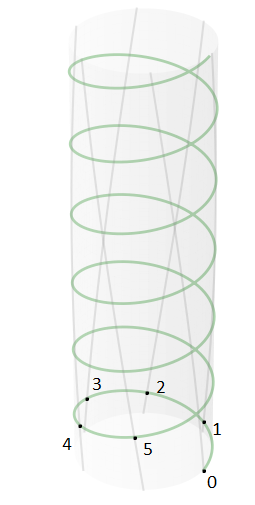
\includegraphics[width=0.3\textwidth]{phase_cylinder.png}
\caption{Намотка числовой прямой на цилиндр при $m=6$:
каждые $6$ шагов спираль поднимается на один виток.}
\label{fig:cylinder}
\end{figure}

\begin{definition}[Фазовая плоскость]\label{def:phase-plane}
Если «разрезать» цилиндр вдоль образующей и развернуть его на плоскость,
спираль превращается в прямоугольную сетку.
Каждое число $n$ имеет координаты $(v(n),h(n))$:
\begin{itemize}
  \item $v(n)\in\{0,\dots,m-1\}$ — \emph{фаза} (горизонтальная координата),
  \item $h(n)\in\Z$ — \emph{высота} (вертикальная координата).
\end{itemize}
Таким образом получаем \emph{фазовую плоскость}, которая является периодической
по фазе с периодом $m$.
\end{definition}

\begin{remark}[Пример при $m=6$]
Числа $0,1,\dots,5$ образуют первый ряд на высоте $h=0$,
числа $6,7,\dots,11$ — второй ряд на высоте $h=1$, и так далее.
Все числа с одинаковой фазой лежат на одной \emph{вертикали}.
\end{remark}

\begin{figure}[H]
\centering
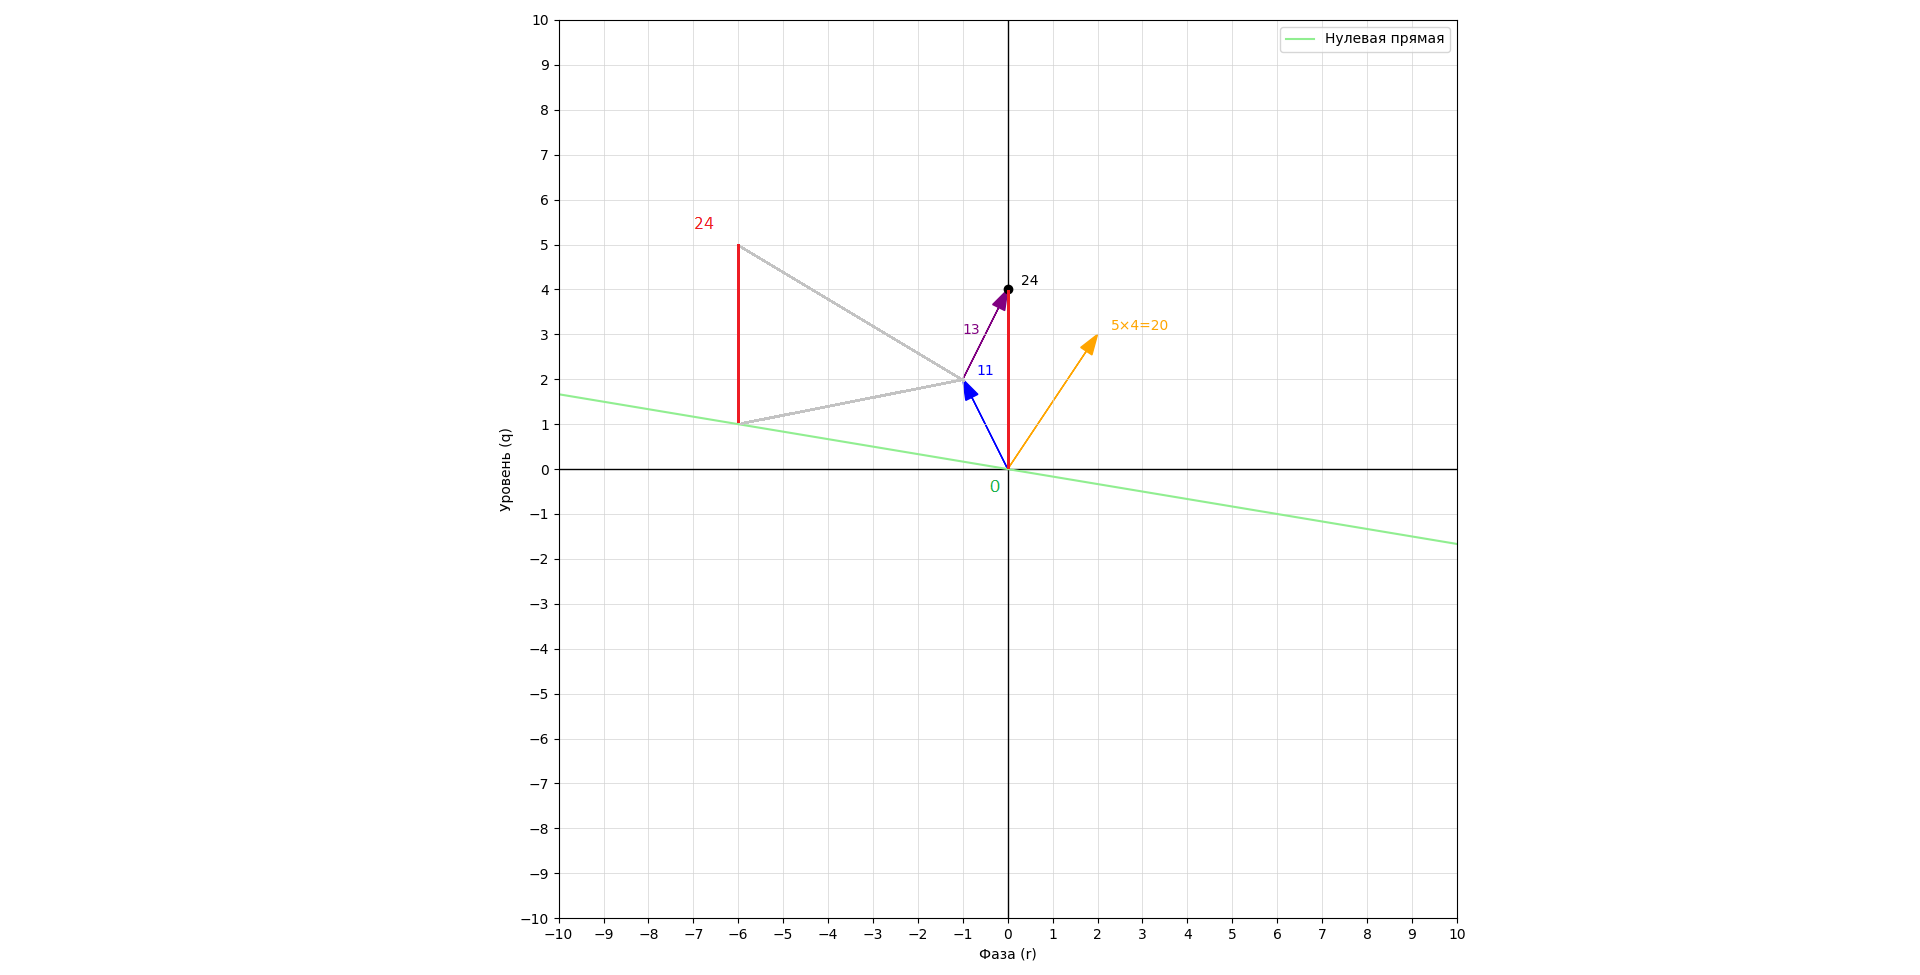
\includegraphics[width=1\textwidth]{phase_plane.png}
\caption{Фазовая плоскость при $m=6$: горизонтальные линии соответствуют высотам,
вертикали — фиксированным фазам.}
\label{fig:phase-plane}
\end{figure}

\section{Векторизация и операции по фазам}

\begin{property}
Каждое число $n$ сопоставляется точке $(v(n),h(n))$ на фазовой плоскости.
При увеличении $n$ на $m$ фаза $v$ остаётся той же, а высота $h$ увеличивается на $1$.
Последовательность чисел с фиксированной фазой образует вертикальный
вектор $(0,1)$; переход по числовой прямой соответствует сложению векторов.
\end{property}

\begin{example}
При $m=6$: переход $8 \to 14$ даёт $(2,1)\to(2,2)$, то есть сдвиг $(0,1)$.
А переход $8 \to 9$ даёт $(2,1)\to(3,1)$, то есть сдвиг $(+1,0)$.
\end{example}

\begin{property}
На фазовой плоскости корректно определены стандартные векторные операции:
\[
(u_1,h_1)+(u_2,h_2)=(u_1+u_2 \bmod m,\,h_1+h_2),\qquad
k\cdot(u,h)=(ku \bmod m,\,kh).
\]
Можно также ввести скалярное произведение $(u_1,h_1)\cdot(u_2,h_2)=u_1u_2+h_1h_2$.
\end{property}

\begin{example}
При $m=6$: $(2,1)+(3,2)=(5,3)$, а $2\cdot(2,1)=(4,2)$.
\end{example}

\begin{property}
Умножение по модулю $m$ и возведение в степень соответствуют линейному действию по фазе:
\[
v \mapsto kv \pmod m.
\]
\end{property}

\begin{example}
Для простого $p=7$ и $a=3$:
\[
1,2,3,4,5,6 \ \mapsto\ 3,6,2,5,1,4,
\]
то есть перестановка фаз. Отсюда $3^6\equiv 1\pmod 7$ (малая теорема Ферма).
\end{example}

\begin{property}
Если $A+B\equiv C\ (\bmod m)$, то на фазовой плоскости три точки
$(v(A),h(A)),\ (v(B),h(B)),\ (v(C),h(C))$ связаны линейным соотношением по фазе,
а по высоте различаются только сдвигами. Фазовая плоскость
естественно кодирует линейные факторы сравнений.
\end{property}

\begin{example}
При $m=6$: $1+2\equiv 3\pmod 6$.
Точки $(1,0),(2,0),(3,0)$ образуют минимальный треугольник,
который повторяется на всех высотах.
\end{example}

\begin{property}
Прямые $pk$ (для простого $p$) проходят через простое число $p$ единично.
Дальше они пересекаются либо на фазе $p^2$ (чётная степень),
либо на произведении $pq$, где они встречаются с прямой $qk$.
\end{property}

\begin{example}
Для $p=5$ и $q=7$:
\[
5^1=5 \ (\text{фаза }5),\quad
5^2=25\equiv 1 \ (\text{фаза }1),\quad
5\cdot 7=35 \ (\text{точка пересечения прямых } 5k \text{ и } 7k).
\]
\end{example}

\begin{property}
Последовательность степеней простого $p^k$ распределяется по фиксированному множеству фаз.
Например, при $m=6$:
\[
5^{2k}\equiv 1\pmod 6,\qquad 5^{2k+1}\equiv 5\pmod 6.
\]
То есть чётные степени всегда лежат в фазе $1$, нечётные — в фазе $5$.
\end{property}

\begin{example}
$5,25,125,625,\dots$ дают чередование фаз $5,1,5,1,\dots$
\end{example}

\begin{property}
Для $m=6$ все простые числа $p>3$ лежат только в двух классах вычетов:
\[
p\equiv 1 \pmod 6 \quad \text{или} \quad p\equiv 5 \pmod 6.
\]
Исключения составляют лишь $p=2$ и $p=3$, так как они являются делителями модуля.
\end{property}

\begin{example}
Простые начинают распределяться так:
\[
5\equiv 5,\quad 7\equiv 1,\quad 11\equiv 5,\quad 13\equiv 1 \pmod 6.
\]
Таким образом простые после $3$ чередуются между фазами $1$ и $5$.
\end{example}

\begin{remark}
Это свойство отражает мультипликативную структуру: произведения чисел из фаз $1$ и $5$
остаются в этих же фазах. Остальные частные случаи следуют из стандартной модульной арифметики
и потому здесь не перечисляются.
\end{remark}



\section{Минимальный треугольник и структура по $BC$}

\begin{definition}[Минимальный треугольник]
Пусть $A,B>0$ и $C=A+B$. Будем называть \emph{минимальным треугольником} исходную тройку $(A,B,C)$,
в которой $A$ и $B$ образуют базис (рёбра), а $C$ — диагональ. Все производные тройки данного класса
получаются сдвигами вдоль тех же прямых $Bk$ и $Ck$:
\[
(A,\;B_k,\;C_k),\qquad B_k:=B+k\cdot BC,\quad C_k:=C+k\cdot BC,\quad k\in\Z.
\]
\end{definition}

\begin{lemma}[Формулы для сдвигов и сохранение прямых]\label{lem:BC-formulas}
Для всякого $k\in\Z$ выполнено
\[
A+B_k=C_k,\qquad B\mid B_k,\quad C\mid C_k,
\]
причём
\[
B_k=B(1+kC),\qquad C_k=C(1+kB).
\]
\end{lemma}

\begin{proof}
Из определений $B_k=B+k\cdot BC=B(1+kC)$ и $C_k=C+k\cdot BC=C(1+kB)$, откуда делимость $B\mid B_k$ и $C\mid C_k$.
Равенство $A+B_k=C_k$ следует напрямую:
\[
A+B_k=A+B+k\cdot BC=C+k\cdot BC=C_k.
\]
\end{proof}

\begin{proposition}[Структура семейства по шагу $BC$]\label{prop:family}
Множество всех троек данного класса есть именно $\{(A,B_k,C_k):k\in\Z\}$.
\end{proposition}

\begin{proof}
Лемма \ref{lem:BC-formulas} даёт включение $\subseteq$: каждая такая тройка удовлетворяет $A+B_k=C_k$ и не
сходит с прямых $Bk$, $Ck$. Обратно, пусть $(A,\widetilde B,\widetilde C)$ удовлетворяет $A+\widetilde B=\widetilde C$ и
$\widetilde B\in B\Z$, $\widetilde C\in C\Z$. Тогда существуют $u,v\in\Z$ со $\widetilde B=Bu$, $\widetilde C=Cv$.
Из $A+Bu=Cv$ вытекает $Bu-Cv=-A$. Поскольку $C=A+B$, получаем $Bu-C(A+B)=-A$, то есть
$Bu-CB-C A=-A$, эквивалентно $B(u-CB)=A(C-1)$. Так как $A,B,C$ фиксированы, из этой линейной связи
существует единственное $k\in\Z$ с $u=1+kC$ и $v=1+kB$, т.е. $\widetilde B=B_k$, $\widetilde C=C_k$.
\end{proof}

\begin{theorem}[Минимальный треугольник по радикалу: существование и единственность]\label{thm:minimal-rad}
Обозначим $R(k):=\rad\!\big(B_kC_k\big)$. Тогда:
\begin{enumerate}[label=\textup{(\alph*)}]
\item \label{item:a} Для всякого $k\in\Z$ выполнено
\[
R(k)\;=\;\rad\!\big(BC\big)\cdot
\frac{\rad\!\big((1+kC)(1+kB)\big)}{\rad\!\big(\gcd\big(BC,(1+kC)(1+kB)\big)\big)}
\;\ge\;\rad\!\big(BC\big).
\]
В частности, новые простые в $B_k$ и $C_k$ могут появиться только из множителей $(1+kC)$ и $(1+kB)$.
\item \label{item:b} Минимум $R(k)$ достигается при $k=0$ и равен $\rad(BC)$.
\item \label{item:c} Если для некоторого $k\neq 0$ выполнено $R(k)=\rad(BC)$, то множества простых делителей
$B_kC_k$ и $BC$ совпадают (никаких новых простых не появилось и ни один из имеющихся не исчез);
такие случаи эквивалентны исходной тройке. В этом смысле минимальный треугольник единственен в классе.
\end{enumerate}
\end{theorem}

\begin{proof}
Из леммы \ref{lem:BC-formulas} имеем факторизации $B_k=B\,(1+kC)$ и $C_k=C\,(1+kB)$.
Радикал произведения равен радикалу произведения радикалов с учётом делителей, общих с $BC$.
Отсюда формула в \ref{item:a} и неравенство $R(k)\ge\rad(BC)$. При $k=0$ получаем ровно $R(0)=\rad(BC)$,
что даёт пункт \ref{item:b}. Если $R(k)=\rad(BC)$ при $k\neq 0$, то ни $(1+kC)$, ни $(1+kB)$
не привнесли новых простых (их простые делители целиком содержатся в $BC$), и ни один простой из $BC$
не «исчез» — следовательно, множества простых совпадают; это и есть пункт \ref{item:c}.
\end{proof}

\begin{example}[Минимальный треугольник $1+2=3$]
Базовая тройка $(1,2,3)$ является минимальным треугольником: $A=1$, $B=2$, $C=3$.
Все остальные тройки этого класса получаются сдвигами
\[
(1,\,2+6k,\,3+6k),\qquad k\in\Z.
\]
Например: $(1,2,3)$, $(1,8,9)$, $(1,14,15)$, $(1,20,21)$ и т.д.
\end{example}

\begin{remark}[Связь с гипотезой ABC]
Минимальный треугольник задаёт базовую структуру, от которой порождаются все остальные тройки класса.
Именно с таких конфигураций удобно начинать анализ качества в духе гипотезы ABC. 
Далее мы введём понятие \emph{провала радикала}, чтобы формализовать этот анализ.
\end{remark}


\section{Провал радикала}

\begin{definition}[Провал радикала]
Для семейства $(A,B_k,C_k)$, задаваемого шагом $BC$, будем говорить,
что возникает \emph{провал радикала}, если при переходе $k \mapsto k+1$
радикал $\rad(A B_{k+1} C_{k+1})$ оказывается меньше, чем на предыдущем шаге.
\end{definition}

\begin{theorem}[Нижняя граница провала]
Пусть $(A,B,C)$ — минимальный треугольник. Тогда для всех $k\in\Z$
\[
\rad(A B_k C_k)\ \ge\ \rad(ABC).
\]
Иными словами, никакой провал радикала не может опуститься ниже радикала
исходного минимального треугольника.
\end{theorem}

\begin{proof}
Мы движемся вдоль прямых $Bk$ и $Ck$, то есть $B\mid B_k$ и $C\mid C_k$ для всех $k$.
Следовательно, все простые делители $B$ и $C$ сохраняются во всех $B_k$ и $C_k$.
А значит, множество простых в $\rad(ABC)$ всегда содержится в множестве простых
в $\rad(A B_k C_k)$, и падение ниже $\rad(ABC)$ невозможно.
\end{proof}

\begin{remark}[Статистическое наблюдение]
Хотя радикал минимального треугольника может встретиться максимум один–два раза,
далее нижняя граница провалов постепенно растёт. Например:
\[
(1,2,3)\ \leadsto\ \rad=6,\qquad
(1,80,81)\ \leadsto\ \rad=30,\qquad
\text{следующие уровни ещё выше.}
\]
Таким образом, провалы радикала существуют, но они всегда ограничены снизу,
и этот минимальный уровень со временем увеличивается.
\end{remark}


\section{Исторический контекст и гипотеза щита}

Наше рассуждение опирается на несколько классических идей:

\begin{itemize}
  \item \textbf{Гипотеза Лежандра} (ок.~1798): в каждом интервале $[n^2,(n+1)^2]$ содержится хотя бы одно простое.
  \item \textbf{Гипотеза простых близнецов} (Харди–Литлвуд, 1923): существует бесконечно много пар простых $(p,p+2)$ и даже предсказана их асимптотическая плотность.
  \item \textbf{Ситовые методы} (Халберстам–Рихерт, Иванець–Ковальски и др.): позволяют оценивать выживаемость кандидатов в простые числа при отсечке малых делителей.
\end{itemize}

Идея \emph{гипотезы щита} возникла как комбинация этих направлений. 
Рассмотрим окно
\[
  I_p = [p^2,(p+2)^2],
\]
где $(p,p+2)$ — пара близнецов. Оно обладает двумя свойствами:
(1) оно достаточно короткое, чтобы проследить комбинаторику кандидатов; 
(2) простые $>p$, а также сами $p$ и $p+2$, не влияют на числа внутри $I_p$. 
Отсюда естественно попытаться оценить, насколько часто кандидаты внутри $I_p$ уничтожаются малыми простыми. 

\begin{hypothesis}[Гипотеза щита]
Для всякой пары простых близнецов $(p,p+2)$ интервал
\[
I_p=[p^2,(p+2)^2]
\]
содержит хотя бы одну пару простых близнецов $(q,q+2)$.
\end{hypothesis}

\section{Две комбинаторные леммы}

\begin{lemma}[дефицит покрытия]
Пусть $I_p=[p^2,(p+2)^2]$. Тогда покрытие $I_p$ числами с делителем $<p$ строго меньше $|I_p|$. 
Следовательно, в $I_p$ существует число без делителей $<p$ (новый простой $\ge p$).
\end{lemma}

\begin{lemma}[двойное сито]\label{lem:double-sieve}
Рассмотрим пары $(n,n+2)$, $n,n+2\in I_p$. 
При отсечке делителей до $z=\sqrt p$ в $I_p$ остаётся $\gg |I_p|/(\ln p)^2$ пар $(n,n+2)$, у которых нет малых делителей. 
Среди них существуют кандидаты на простые близнецы.
\end{lemma}

Эти две простые леммы вместе объясняют, почему интервал $I_p$ выступает как «щит»: старые простые не могут полностью закрыть все кандидаты, а двойное сито гарантирует наличие большого числа пар, которые выживают. Именно это мотивирует формулировку гипотезы щита.

\section{Фазово-высотная формулировка гипотезы Гольдбаха}

Введём понятие \emph{высоты} относительно шага $H\in\mathbb{N}$:
\[
x = H\,h_H(x) + r_H(x), \qquad h_H(x)=\Big\lfloor \tfrac{x}{H}\Big\rfloor,\;\;0\le r_H(x)<H.
\]
Здесь $h_H(x)$ называется \emph{высотой} числа $x$, а $r_H(x)$ — \emph{остатком по горизонтали}.

\begin{lemma}[Аддитивность высот]
Для $N=A+B$ имеем
\[
h_H(N) = h_H(A)+h_H(B)+c_H(A,B),
\]
где перенос $c_H(A,B)\in\{0,1\}$ равен $1$ тогда и только тогда, когда $r_H(A)+r_H(B)\ge H$.
\end{lemma}

Совместив это с фазовой классификацией по модулю $6$, получаем простое, но ключевое ограничение:

\begin{lemma}[Фазово-высотная лемма для Гольдбаха]
Для всякого чётного $N>4$ верно:
\[
N \equiv 2 \pmod{6} \;\Rightarrow\; N=(6k+1)+(6k'+1),
\]
\[
N \equiv 0 \pmod{6} \;\Rightarrow\; N=(6k+1)+(6k'-1),
\]
\[
N \equiv 4 \pmod{6} \;\Rightarrow\; N=(6k-1)+(6k'-1).
\]
Иными словами, всякое голдбаховское разложение фиксируется одновременно по вертикали (сумма высот)
и по горизонтали (фаза $N$).
\end{lemma}

Таким образом, гипотеза Гольдбаха приобретает жёсткую структуру: для заданного чётного $N$ остаётся лишь
проверить наличие простых на предписанной высоте и в предписанной фазе. Это позволяет рассматривать задачу
не через массовый анализ распределения простых, а через дискретную геометрию фазовых вертикалей.

\section*{Заключение}
В работе предложена геометрическая модель на основе фазовой намотки и введено понятие высоты, 
которая позволяет унифицировать взгляд на несколько классических задач теории чисел. 
Мы не ставили целью дать окончательные доказательства, а показали, как разные гипотезы 
получают наглядное и структурное представление в рамках одной схемы.

\begin{itemize}
  \item Гипотеза ABC традиционно формулируется через радикалы чисел и тройки решений $a+b=c$. В нашей модели она получает наглядное представление как диофантовое уравнение в геометрической схеме фазовых координат. Насколько нам известно, именно такой ракурс отдельно в литературе не выделялся
  \item Для гипотезы Гольдбаха переход к фазам и высотам позволяет трактовать задачу 
  не как «случайное пересечение простых», а как \emph{неизбежную структуру}: 
  каждая чётная вершина попадает в строго определённую фазу и фиксируется суммой высот простых.
  \item Гипотеза «Щита» возникла благодаря введению вертикалей: 
  стало видно, что в фиксированном окне часть вертикалей систематически занята простыми числами, 
  причём на одной вертикали. Первичный численный анализ до $10^7$ (и частично до $10^{10}$) 
  подтвердил это наблюдение: вертикали действительно повторяются устойчиво. 
  На этой основе и была сформулирована сама гипотеза — как это обычно и происходит 
  при рождении новых идей в теории чисел.
\end{itemize}

Таким образом, мы показали, что единая конструкция (фазы и высоты) позволяет по-новому взглянуть 
на три значимые гипотезы современной теории чисел. С одной стороны, строгие доказательства остаются открытыми; 
с другой стороны, предложенный подход выявляет скрытую структуру распределения простых и задаёт 
новые перспективы для дальнейших исследований.

\begin{thebibliography}{99}

\bibitem{ApostolANT}
T.~M.~Apostol, \emph{Introduction to Analytic Number Theory}. Springer, 1976.

\bibitem{HardyWright}
G.~H.~Hardy, E.~M.~Wright, \emph{An Introduction to the Theory of Numbers}. 6th ed., Oxford Univ. Press, 2008.

\bibitem{HardyLittlewood}
G.~H.~Hardy, J.~E.~Littlewood, ``Some problems of Partitio Numerorum III: On the expression of a number as a sum of primes,'' 
\emph{Acta Math.}, 44 (1923), 1–70.

\bibitem{HalberstamRichert}
H.~Halberstam, H.-E.~Richert, \emph{Sieve Methods}. Academic Press, 1974.

\bibitem{IwaniecKowalski}
H.~Iwaniec, E.~Kowalski, \emph{Analytic Number Theory}. AMS Colloquium Publ. 53, 2004.

\end{thebibliography}


\end{document}
